%%%%%%%%%%%%%%%%%%%%%%%%%%%%%%%%%%%%%%%%%%%%%%%%%%%%%%%%%%%%%%%%%
\chapter{Environment Setup}
\label{ch:environment-setup}
%%%%%%%%%%%%%%%%%%%%%%%%%%%%%%%%%%%%%%%%%%%%%%%%%%%%%%%%%%%%%%%%%

This chapter walks through the installation of all software required
for the \ProjectName{} project. Work through the required
sections in order before the first session. Optional sections can be
completed at any time. The instructions are written primarily for
Windows but include equivalent steps for macOS and Linux throughout.

\vs
\noindent
Familiarity with the command line and with file paths is helpful but
not required here. These concepts are covered fully in
Chapter~\ref{ch:cli-scripting}, which you can read after completing
this chapter.
\vs

%================================================================
\section{Required: Install Python}\label{sec:python}
%================================================================

Install any recent Python version from \href{https://www.python.org/downloads/}{https://www.python.org/downloads/}. Go to your downloads and double click on the install file to start installation. By default the Python installer for Windows places its executables in the user's AppData directory, so that it doesn't require administrative permissions. This works for most scenarios. If you're the only user on the system, you might want to place Python in a higher-level directory (e.g. \texttt{C:\textbackslash Python} or \texttt{/usr/local/bin}) to have a shorter path to the binaries (sometimes you will need that). Depending on your preferences, either select ``\textit{Install Now}'' or ``\textit{Customized installation}'' (my preference). Please make sure you select ``\textit{Add python.exe to path}''; this will save you a few headaches later.

\begin{figure}[htbp]
	\centering
	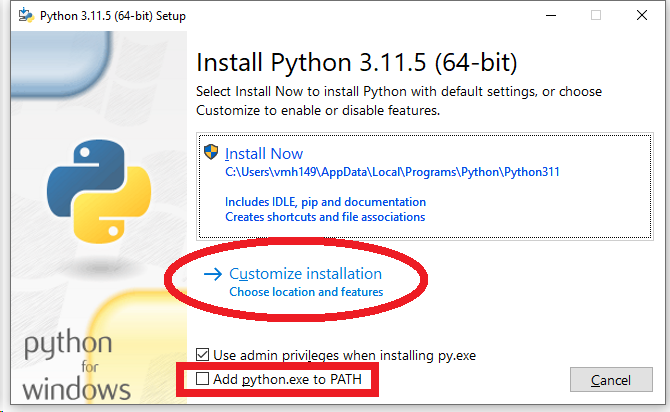
\includegraphics[width=0.65\textwidth]{../images/envsetup-3-1.png}
	\caption{Python installer showing the ``Add python.exe to PATH'' checkbox at the bottom.}
	\label{fig:envsetup-3-1}
\end{figure}

In the window ``Optional Features'' select all features

\begin{figure}[htbp]
	\centering
	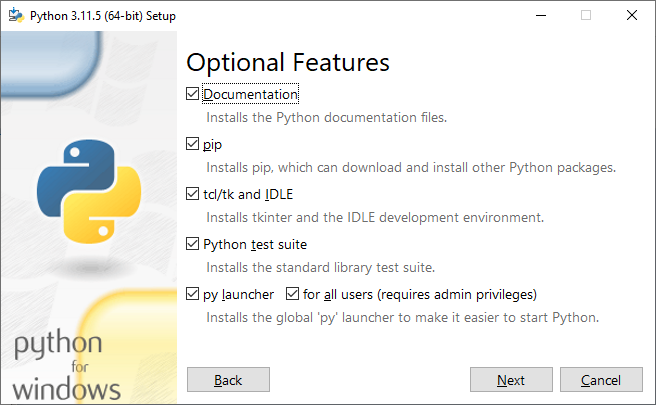
\includegraphics[width=0.65\textwidth]{../images/envsetup-4-1.png}
	\caption{Python Optional Features screen: select all features.}
	\label{fig:envsetup-4-1}
\end{figure}

Select ``\textit{Install Python X.XX for all users}'' if you can and want. This requires administrative privileges. Select the folder of your choice for the install location.

\begin{figure}[htbp]
	\centering
	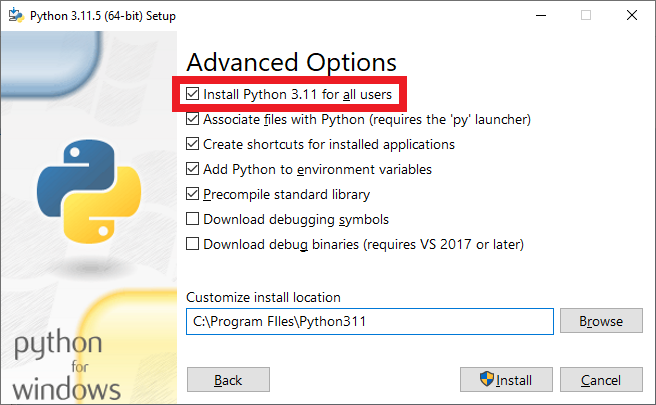
\includegraphics[width=0.65\textwidth]{../images/envsetup-4-2.png}
	\caption{Python Advanced Options screen showing ``Install for all users'' selected.}
	\label{fig:envsetup-4-2}
\end{figure}

For PC: If you did not add \texttt{python.exe} to the PATH during installation, wait until the installation is complete. Then open File Explorer and right-click on ``This PC.'' Select ``Properties'' from the context menu. In the System window that opens, click on ``Advanced system settings'' in the left-hand sidebar. In the new window, ensure the ``Advanced'' tab is selected and click the ``Environment Variables'' button near the bottom. Under the ``System variables'' section, find and double-click on the variable named ``Path.'' This will open a window where you can add the path to the Python executable manually.

\vs

For Mac: If you did not ensure Python was added to your system's PATH during installation, you can manually do so using the following steps on a Mac. After installation is complete, open the Terminal application. Enter the command \texttt{which python3} or \texttt{which python} to find the path to the installed Python binary. Copy that path. Then open your shell configuration file in a text editor. This will typically be \texttt{\~{}/.zshrc} if you are using the Zsh shell (default on newer versions of macOS) or \texttt{\~{}/.bash\_profile} if you are using Bash. Add the line \texttt{export PATH="/path/to/python:\$PATH"}, replacing \texttt{/path/to/python} with the path you copied. Save the file and close the editor. In the Terminal, run \texttt{source \~{}/.zshrc} or \texttt{source \~{}/.bash\_profile} depending on the file you edited, so the new PATH is loaded into your environment.

%================================================================
\section{Optional (but \underline{strongly} encouraged): Install a \LaTeX{} Distribution}\label{sec:latex-install}
%================================================================

\LaTeX{} is a high-quality typesetting system designed for the creation of 
technical and scientific documents. Rather than formatting text visually, 
authors write plain-text source files using a markup language that describes 
the structure and meaning of the content (such as sections, equations, 
and references). These source files are then compiled into professionally 
formatted documents (typically PDFs). \LaTeX{} excels at typesetting 
equations, managing cross-references, and producing consistent, 
publication-quality output, making it the standard tool for many fields 
in science, engineering, and mathematics.

\begin{infobox}
	\LaTeX{} is particularly well suited for interaction with Large Language Models
\end{infobox}


\LaTeX{} is particularly well suited for interaction with Large Language Models 
(LLMs) because it is a purely textual, declarative markup language that closely 
resembles structured source code. Unlike binary document formats (e.g., Word or PDF), 
a \LaTeX{} document exposes its full logical structure---sections, equations, 
environments, and references---in plain text. This makes it directly 
interpretable, editable, and generatable by LLMs, which are fundamentally 
trained on and optimized for text and code. As a result, LLMs can reliably 
assist with tasks such as drafting mathematical content, refactoring structure, 
verifying notation, and even debugging compilation issues. In this sense, 
\LaTeX{} serves as a natural interface between human mathematical reasoning 
and machine-assisted generation, enabling precise, reproducible, and automatable 
document workflows.

\LaTeX{} is required if you intend to compile \texttt{.tex} documents
locally. The program's documents are maintained as \LaTeX{} source files
in the repository. For authoring and compiling your own
documents, install the distribution for your platform.


\begin{table}[htbp]
\centering
\caption{Recommended \LaTeX{} distributions by platform}
\label{tab:latex-distros}
\begin{tabular}{llp{7.5cm}}
\toprule
\textbf{Platform} & \textbf{Distribution} & \textbf{Download} \\
\midrule
Windows & MiKTeX & \url{https://miktex.org} \\
macOS & MacTeX & \url{https://www.tug.org/mactex/} \\
Linux (Ubuntu/Debian) & TeX Live & \texttt{sudo apt install texlive-latex-extra texlive-fonts-recommended latexmk} \\
\bottomrule
\end{tabular}
\end{table}

Verify the installation on any platform with:

\begin{verbatim}
pdflatex --version
\end{verbatim}

\vs
\noindent
Usage of \LaTeX{} for document preparation, including a mathematics
notation cheat sheet, is covered in Chapter~\ref{ch:latex}.
\vs

%================================================================
\section{Required: Install Visual Studio Code (VSC)}\label{sec:vsc}
%================================================================

\textbf{If you are new to Python, install \href{https://code.visualstudio.com}{Visual Studio Code} (VSC)}: There are many options to write Python code, and you could have a favorite one. I must pick one to deliver instruction, and experience has shown me that VSC offers the least amount of friction.

\vs

In VSC, there are two main options: ``\textit{User Installer}'' and ``\textit{System Installer}''. Use the User Installer if you want to install only for the current user. For all users, use System installer; I prefer this choice because it installs VSC in \texttt{C:\textbackslash Program Files\textbackslash Microsoft VS Code}.

\vs

Visual Studio Code is available for Windows, macOS, and Linux; an identical open-source alternative called VSCodium is available at \url{https://vscodium.com}.

%================================================================
\section{Required: Visual Studio Code extensions}\label{sec:extensions}
%================================================================

Select the Extensions icon on the left and install the following Visual Studio Code libraries

\begin{enumerate}
	\item \textbf{Required}: Python extension for Visual Studio Code.

	\item \textbf{Optional}: Also install Jupyter (this also installs Pylance, Jupyter Keymap, Jupyter Notebook Renderers, Jupyter SlideShow). Pay attention to the publisher of the extension; use the ones by Microsoft.

	\begin{figure}[htbp]
		\centering
		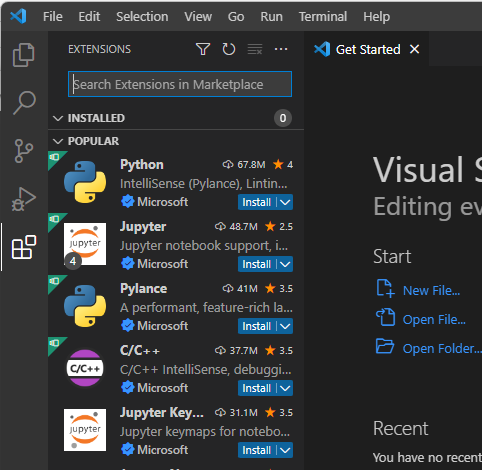
\includegraphics[width=0.7\textwidth]{../images/envsetup-5-1.png}
		\caption{VS Code Extensions marketplace showing the Python and Jupyter extensions by Microsoft.}
		\label{fig:envsetup-5-1}
	\end{figure}

	\item \textbf{Optional}: Install C/C++ for Visual Studio Code, C/C++ Themes \& C/C++ Extension Pack.

	\item \textbf{Optional}: Install the extension ``\textbf{LaTeX Workshop}'' by James Yu. This extension provides syntax highlighting, live preview, and one-click build. Its use is described in Section~\ref{sec:latex-workshop}.

	\begin{figure}[htbp]
		\centering
		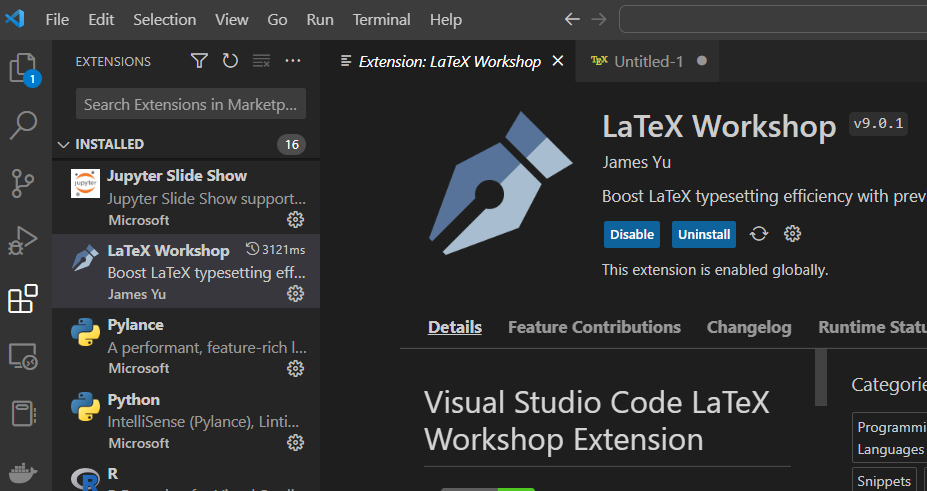
\includegraphics[width=0.7\textwidth]{../images/envsetup-6-1.png}
		\caption{LaTeX Workshop extension page in VS Code.}
		\label{fig:envsetup-6-1}
	\end{figure}
\end{enumerate}

%================================================================
\section{Optional: Windows Terminal}\label{sec:terminal}
%================================================================

For Windows users, install \href{https://apps.microsoft.com/detail/windows-terminal}{Windows Terminal}. This Microsoft app allows you to use a multi document window with tabs for different command consoles like PowerShell, Ubuntu, DOS, Git, etc. You will need this if you want to complete the steps related to Linux in the next section of this document.

%================================================================
\section{Required: Install Git}\label{sec:git}
%================================================================

Install \href{https://gitforwindows.org}{Git for Windows}. For Mac, install \href{https://git-scm.com/download/mac}{Git for Mac}. Linux also has a version available. In the second screen, select Visual Studio Code as your Git editor. Use all other default options.

\begin{figure}[htbp]
	\centering
	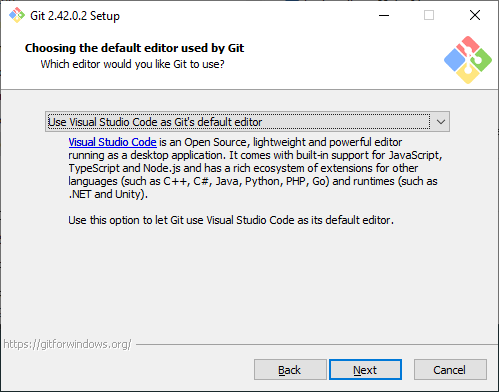
\includegraphics[width=0.6\textwidth]{../images/envsetup-2-1.png}
	\caption{Git setup screen showing Visual Studio Code as the default editor.}
	\label{fig:envsetup-2-1}
\end{figure}

%================================================================
\section{Required: Open Git Bash (or any terminal)}\label{sec:gitbash}
%================================================================

The command line allows you to control your computer by typing instructions, providing precise access to files and system features. For example, typing \texttt{ls} on a Unix-like system such as Linux or macOS lists the files and directories in the current location, such as \texttt{ls /home/user/Documents} to display the contents of the Documents folder. On Windows, the \texttt{dir} command serves the same function, so \texttt{dir C:\textbackslash Users\textbackslash Alice\textbackslash Desktop} shows what is on the Desktop. To move between directories, the \texttt{cd} command is used; \texttt{cd Downloads} changes the working directory to Downloads, while \texttt{cd ..} moves one level up. These commands allow efficient navigation and inspection of the file system through the terminal.

\vs

Now that Git is installed, clone the \ProjectName{} 
repository. Open Git Bash (Windows) or a terminal (macOS/Linux),
navigate to the folder where you want to store the project, and run:

{\ttfamily \noindent
git clone \ProjectGit.git
}

This creates a folder called \texttt{\ProjectFolder} containing all
workshop materials. You only need to do this once. To update your
local copy later, navigate into the folder and run \texttt{git pull}.

%================================================================
\section{Required: Open the \ProjectName{} project in Visual Studio Code}\label{sec:vscstart}
%================================================================

To open the \ProjectName{} project in VSC, open a terminal, navigate into the
\texttt{\ProjectFolder} folder you cloned in the previous section,
and run:

{\ttfamily \noindent
cd \ProjectFolder \\
code .
}

The period after \texttt{code} instructs VSC to use the current folder
as the working folder. All workshop files will be visible in the VSC
file explorer.

%================================================================
\section{Required: Install Python libraries}\label{sec:libraries}
%================================================================

Python libraries for the data challenge are installed inside a virtual
environment. Complete Chapter~\ref{ch:python-environments} to set up
your environment, then install the required libraries as described there.

%================================================================
\section{Optional: Jupyter Notebook}\label{sec:jupyter}
%================================================================

\textbf{Optional}: Now, create a Jupyter Notebook.

\begin{enumerate}
	\item Abundant relevant information regarding Jupyter in VSC is available at \href{https://code.visualstudio.com/docs/datascience/jupyter-notebooks}{https://code.visualstudio.com/docs/datascience/jupyter-notebooks}

	\item Activate the environment you want to use (see Chapter~\ref{ch:python-environments}).

	\item You need to attach the kernel of your virtual environment. For example, if I have a virtual environment called venn:

	\begin{verbatim}
	python -m ipykernel install --user --name=venn
	\end{verbatim}

	\item Open VS Code in your project folder (see Section~\ref{sec:vscstart}).

	\item In VSC, run the command \texttt{Create:New Jupyter Notebook} from the Command Palette (Ctrl+Shift+P) or by creating a new .ipynb file in your workspace.

	\item You might receive a Security Alert regarding the firewall. Allow access.

	\begin{figure}[htbp]
		\centering
		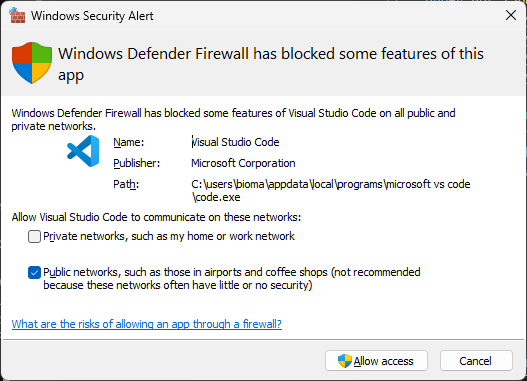
\includegraphics[width=0.6\textwidth]{../images/envsetup-14-1.png}
		\caption{Windows Defender Firewall alert: allow access for Visual Studio Code.}
		\label{fig:envsetup-14-1}
	\end{figure}

	\item After you enter a command, you might see the following message:

	\begin{figure}[htbp]
		\centering
		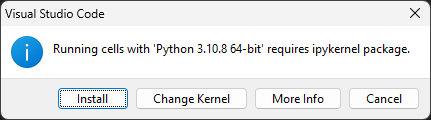
\includegraphics[width=0.55\textwidth]{../images/envsetup-14-2.png}
		\caption{VS Code prompt to install the ipykernel package: click Install.}
		\label{fig:envsetup-14-2}
	\end{figure}

	Install it.
\end{enumerate}

%================================================================
\section{Optional: Python commands in Terminal}\label{sec:pythonterminal}
%================================================================

Finally, you can simply enter Python commands in the Terminal. Open a Command Prompt and type the following command:

\begin{verbatim}
python
\end{verbatim}

This will allow you to enter python commands, e.g. \texttt{1+1}

%================================================================
\section{Troubleshoot}\label{sec:troubleshoot}
%================================================================

The following errors have been reported by previous participants.
If you encounter a different issue, consult the \ProjectName{} repository
issue tracker at \url{\ProjectGit/issues}.

\vs

As reported by Lorena Roa de La Cruz, you could see an error when trying to activate a virtual environment. This is due to configuration of permissions. If this happens, run the command:

\begin{verbatim}
Set-ExecutionPolicy -ExecutionPolicy RemoteSigned -Scope CurrentUser
\end{verbatim}

After that, run the script \texttt{activate}.

\begin{figure}[htbp]
	\centering
	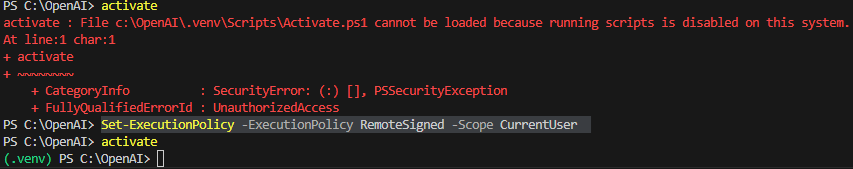
\includegraphics[width=0.85\textwidth]{../images/envsetup-12-1.png}
	\caption{PowerShell execution policy error and fix: running \texttt{Set-ExecutionPolicy} followed by \texttt{activate}.}
	\label{fig:envsetup-12-1}
\end{figure}

%================================================================
\section{Optional: C/C++ compilers}\label{sec:compilers}
%================================================================

If you'd like to code in C or C++, you have several options, including \href{https://gcc.gnu.org}{GCC, the GNU Compiler Collection}, but it requires some effort to install the prerequisites. From Microsoft there is \href{https://visualstudio.microsoft.com/vs/community/}{Visual Studio Community Edition} (VSCE), which encapsulates the complexity of installing multiple compilers (including the .NET framework SDK). I recommend you install VSCE with all ``Workloads'' in ``Web \& Cloud'' and ``Desktop \& Mobile'' (except Python).

%================================================================
\section{Optional: Installing PostgreSQL on Linux}
%================================================================
Many Linux distributions ship with older versions of PostgreSQL in their
default repositories. To install the latest stable version, it is recommended
to use the official PostgreSQL package repository maintained by the
PostgreSQL Global Development Group.

The following procedure installs the most recent stable release on
Ubuntu or Debian systems.

%----------------------------------------------------------------
\subsection{Install Required Utilities}
%----------------------------------------------------------------
First install utilities required to retrieve and verify packages.

\begin{lstlisting}[basicstyle=\footnotesize\ttfamily]
sudo apt update
sudo apt install curl ca-certificates
\end{lstlisting}

%----------------------------------------------------------------
\subsection{Add the PostgreSQL Repository}
%----------------------------------------------------------------
Add the official PostgreSQL repository to the system package sources.

\begin{lstlisting}[basicstyle=\footnotesize\ttfamily]
sudo sh -c 'echo "deb http://apt.postgresql.org/pub/repos/apt \
$(lsb_release -cs)-pgdg main" \
> /etc/apt/sources.list.d/pgdg.list'
\end{lstlisting}

%----------------------------------------------------------------
\subsection{Import the Repository Signing Key}
%----------------------------------------------------------------
Import the PostgreSQL repository signing key.

\begin{lstlisting}[basicstyle=\footnotesize\ttfamily]
curl -fsSL https://www.postgresql.org/media/keys/ACCC4CF8.asc \
| sudo gpg --dearmor -o /usr/share/keyrings/postgresql.gpg
\end{lstlisting}

Update the repository configuration to reference the key.

\begin{lstlisting}[basicstyle=\footnotesize\ttfamily]
sudo nano /etc/apt/sources.list.d/pgdg.list
\end{lstlisting}

Modify the line to read in a single line (the character \textbackslash{}  means line return; it is here just to indicate that all is one line; delete it and join the following three lines of text into a single line):

\begin{lstlisting}[basicstyle=\footnotesize\ttfamily]
deb [signed-by=/usr/share/keyrings/postgresql.gpg] \
http://apt.postgresql.org/pub/repos/apt \
$(lsb_release -cs)-pgdg main
\end{lstlisting}

%----------------------------------------------------------------
\subsection{Install PostgreSQL}
%----------------------------------------------------------------
Update the package index and install the latest PostgreSQL version.

\begin{lstlisting}[basicstyle=\footnotesize\ttfamily]
sudo apt update
sudo apt install postgresql-16
\end{lstlisting}

%----------------------------------------------------------------
\subsection{Verify the Installation}
%----------------------------------------------------------------
Confirm that PostgreSQL was installed successfully.

\begin{lstlisting}[basicstyle=\footnotesize\ttfamily]
psql --version
\end{lstlisting}

The output should indicate the installed PostgreSQL version.

%----------------------------------------------------------------
\subsection{Start the Database Server}
%----------------------------------------------------------------
If the service is not already running, start the PostgreSQL cluster.

\begin{lstlisting}[basicstyle=\footnotesize\ttfamily]
sudo systemctl start postgresql
\end{lstlisting}

Verify the server status:

\begin{lstlisting}[basicstyle=\footnotesize\ttfamily]
sudo systemctl status postgresql
\end{lstlisting}

%----------------------------------------------------------------
\subsection{Access the PostgreSQL Shell}
%----------------------------------------------------------------
To open the PostgreSQL interactive terminal:

\begin{lstlisting}[basicstyle=\footnotesize\ttfamily]
sudo -u postgres psql
\end{lstlisting}

Exit the shell using:

\begin{lstlisting}[basicstyle=\footnotesize\ttfamily]
\q
\end{lstlisting}
